\begin{definition} \cite{hunger}
  The Galois group of a polynomial \(f \in K[x]\) is the group \(Aut_K^F\), where \(F\) is a splitting field of \(f\) over \(K\).
\end{definition}
\begin{theorem} \cite{hunger} Let \(G\) be a Galois group of a polynomial \(f \in K[x]\).
\begin{enumerate}
\item[i)] \(G\) is isomorphic to a subgroup of some symmetric group \(S_n\).
\item[ii)] If \(f\) is separable of degree \(n\), the \(n\) divides \(|G|\) and \(G\) isomorphic to a transitive subgroup of \(S_n\).  \end{enumerate}
\end{theorem}
Because the Galois group \(Aut_K^F\) is a ``group of automorphisms of F which is given by the permutations of the roots Galois group of a polynomial is identified with the subgroup of \(S_n\)'' \cite{hunger}.
\vspace{3mm}

\begin{corollary}
\begin{enumerate}
 \cite{hunger} \item[i)] If the degree of \(f\) is \(2\) then its Galois group \(G \cong {\mathbb{Z}}_2\).
  \item[ii)] If the degree of \(f\) is \(3\) then its Galois group \(G\) is either \(S_3\) or \(A_3\).
  \end{enumerate}
\end{corollary}

\vspace{-2mm}
\section{Galois Group of Cubic polynomials}
\begin{definition} \cite{hunger}
  Let \(K\) be a field with \(char K \neq 2\) and \(f \in K[x]\) a polynomial of degree \(n\) with \(n\) distinct roots \(u_1,u_2,...,u_n\) in some splitting field \(F\) of \(f\) over \(K\). Let \(\Delta = \prod\limits_{i<j}(u_i-u_j) = (u_1-u_2)(u_1-u_3)...(u_{n-1}-u_n) \in F\).\\
  The discriminant of \(f\) is the element \(D= {\Delta}^2\).
\end{definition}

\begin{theorem}
\begin{enumerate}  \cite{hunger}
\item[i)] The discriminant \({\Delta}^2\) of \(f\) actually lies in \(K\).
  \item[ii)] For each \(\sigma \in Aut_K^F < S_n, \sigma\) is an even[resp. odd] if and only if \(\sigma(\Delta) = \Delta\)[resp. \(\sigma(\Delta) = - \Delta\)].
  \end{enumerate}
\end{theorem}
Since \({\Delta}^2 \in K\) and \(\Delta \in F\), and \(K(\Delta)\) is a stable intermediate; in the ``Galois correspondence the subfield \(K(\Delta)\) corresponds to the subgroup \(G \cap A_n\). In particular, \(G\) consists of even permutations if and only if \(\Delta \in K\)'' \cite{hunger}.

\begin{corollary} \cite{hunger}
  If \(f\) is a separable polynomial of degree \(3\), then the Galois group of \(f\) is \(A_3\) if and only if the discriminant of \(f\) is the square of an element of \(K\).
\end{corollary}
\vspace{-3mm}
\begin{theorem} \cite{hunger}
  Let \(K\) be a field of \(char K \neq 2,3 \). If \(f(x)=x^3+bx^2+cx+d \in K[x]\) has three distinct roots in some splitting field, then the polynomial \(g(x)=f(x-b/3) \in K[x]\) has the form \(x^3+p^2+q\) and the discriminant of \(f\) is \(-4p^3-27q^2\).
\end{theorem}
\vspace{-2mm}
\section{Galois Group of Quartic polynomials}
\begin{definition} \cite{hunger} [Resolvant Cubic of a Quartic]
Let \(K, f, F, u_i, V,\) and \(G=Aut_K^F<S_4\) be as in the preceding paragraph and \(\alpha=u_1u_2+u_3u_4,\) \(\beta=u_1u_3+u_2u_4,\) \(\gamma=u_1u_4+u_2u_3\).
The polynomial \( (x- \alpha)(x- \beta)(x- \gamma) \) is called the resolvant cubic of \(f\). The resolvant cubic is actually a polynomial over \(K\).
\end{definition}

Now under ``the Galois correspondence the subfield \(K(\alpha, \beta, \gamma)\) corresponds to the normal subgroup \(V \cap G\)'' \cite{hunger} because \(K(\alpha,\beta,\gamma)\) is a splitting field of the resolvant cubic whose Galois group is a subgroup of \(S_3\) and only normal subgroup \(N\) of \(S_4\) with \(|N| \leq 6\) is \(V\), where \(V=\{(1),(12)(34),(13)(24),(14)(23)\}\).\\
``Hence \(K(\alpha, \beta, \gamma)\) is Galois over \(K\) and \(Aut_K^{K(\alpha, \beta, \gamma)} = G/(G \cap V)\)'' \cite{hunger}.

\begin{remark} \cite{hunger} If \(K\) is a field and \(f = x^4+bx^3+cx^2+dx+e \in K[x]\), then the resolvant cubic of \(f\) is the polynomial \(x^3-cx^2+(bd-4e)x-b^2e+4ce-d^2 \in K[x]\).
\end{remark}

\begin{tcolorbox}[boxsep=-1mm]
\begin{theorem} \cite{hunger}
  Let \(K\) be a field and \(f \in K[x]\) a separable quartic with Galois Group \(G\). Let \(\alpha, \beta, \gamma\) be the roots of the resolvant cubic of \(f\) and let \(m= [K(\alpha, \beta, \gamma) : K]\) then,
\begin{enumerate}
\item[i)] \(m=6 \Longleftrightarrow G=S_4\);
\item[ii)] \(m=3 \Longleftrightarrow G=A_4\);
\item[iii)] \(m=1 \Longleftrightarrow G=V\);
\item[iv)] \(m=2 \Longleftrightarrow G=D_4\) or \(G={\mathbb{Z}}_4\); in this case \(G={\mathbb{Z}}_4\) if \(f\) is irreducible over \(K(\alpha, \beta, \gamma)\) and \(G={\mathbb{Z}}_4\) otherwise.
\end{enumerate}
\end{theorem}
\end{tcolorbox}
This is because we have \([K(\alpha,\beta,\gamma):K] = |G/G \cap V|\).

\section{Galois Group of some Polynomials}
\begin{example} \cite{hunger}
The polynomial is \(f(x)=x^4-2 \in \mathbb{Q}[x]\). This polynomial is irreducible and therefore separable over \(\mathbb{Q}\). The resolvant cubic is \(x^3+8x = x(x+2i\sqrt{2})(x-2i\sqrt{2})\) and \(\mathbb{Q}(\alpha,\beta, \gamma)=\mathbb{Q}(i\sqrt{2})\) has dimension \(2\) over \(\mathbb{Q}\). \(x^4-2\) is irreducible over \(\mathbb{Q}(i\sqrt{2})\) because \(\sqrt[\leftroot{-3}\uproot{3}4]{2} \not\in \mathbb{Q}(i\sqrt{2})\). Therefore the Galois group \(G \cong D_8\).
\end{example}

``Let \(F \subset \mathbb{C}\) be a splitting field over \(\mathbb{Q}\) of \(f(x)=x^4-2 \in \mathbb{Q}[x]\). If \(u\) is the positive real fourth root of 2, then the roots of \(f\) are \(u,\; -u,\; ui,\; -ui\). To find the  Galois group \(G = Aut_{\mathbb{Q}}^F\) of \(f\) which is a subgroup of \(S_4\), we find the permutations of the roots. To do so  we must choose an ordering of the roots, say \(u_1=u\), \(u_2=ui\), \(u_3=-u\), \(u_4= -ui\). The complex conjugation is an \(\mathbb{R}\)-automorphism of \(\mathbb{C}\) which clearly sends:
\(u \mapsto u\), \(-u \mapsto -u\), \(ui \mapsto -ui\) and \(-ui \mapsto ui\). \\
This induces a \(\mathbb{Q}\)-automorphism \(\tau\) of \(F=\mathbb{Q}(u,ui)\). As an element of \(S_4\)'' \cite{hunger}, \(\tau=(24)\).
Now the generator of \(D_8\) containing \(\tau = (24)\) is \(\sigma = (1234)\). We have ``\(F=\mathbb{Q}(u,ui)=\mathbb{Q}(u,i)\),
so every \(\mathbb{Q}\)-automorphism of \(F\) is completely determined by its action on \(u\) and \(i\). Thus the elements of \(G\)
may be described either in terms of \(\sigma\) and \(\tau\) or by their action on \(u\) and \(i\). The information is summarized in the table'' \cite{hunger}
\vspace{2mm}

\begin{table}[h!]
\begin{tabular}{|c|c|c|c|c|c|c|c|c|}
  \hline
  \ & (1) & (24) & (1234) & (13)(24) & (1432) & (12)(34) & (13) & (14)(32) \\
  \ &  & \(\tau\)  & \(\sigma\) & \({\sigma}^2\) & \({\sigma}^3\) & \(\sigma \tau\) & \({\sigma}^2 \tau\) & \({\sigma}^3 \tau\) \\
  \hline
  \(u \mapsto\) & \(u\) & \(u\) & \(ui\) & \(-u\) & \(-ui\) & \(ui\) & \(-u\) & \(-ui\) \\
  \(i \mapsto\) & \(i\) & \(-i\) & \(i\) & \(i\) & \(i\) & \(-i\) & \(-i\) & \(-i\) \\
  \hline
\end{tabular}
\caption{\small Roots permutation table.}
\end{table}

\begin{tikzpicture}

  \node[minimum width=3mm, minimum height=3mm, align=center] (i) {\((1)\)};

  \node[below of=i, minimum width=3mm, minimum height=3mm, align=center, yshift=-10mm] (ss) {\(<{\sigma}^2>\)};

  \node[left of=ss, minimum width=3mm, minimum height=3mm, align=center, xshift=-20mm] (sst) {\(<{\sigma}^2 \tau>\)};

  \node[
  left of=sst,
  minimum width=3mm,
  minimum height=3mm,
  align=center,
  xshift=-20mm
  ] (t) {\(<\tau>\)\>};

  \node[
  right of=ss,
  minimum width=3mm,
  minimum height=3mm,
  align=center,
  xshift=20mm
  ]
  (st) {\(<\sigma\tau>\)};

  \node[
  right of=st,
  minimum width=3mm,
  minimum height=3mm,
  align=center,
  xshift=20mm
  ]
  (ssst) {\(<{\sigma}^3\tau>\)};

  \node[
  below of=ss,
  minimum width=3mm,
  minimum height=3mm,
  align=center,
  yshift=-10mm
  ]
  (s) {\(<\sigma>\)};

  \node[
  left of=s,
  minimum width=3mm,
  minimum height=3mm,
  align=center,
  xshift=-30mm
  ]
  (iss) {\(<(1),{\sigma}^2,\sigma,\tau,{\sigma}^2\tau>\)};

  \node[
  right of=s,
  minimum width=3mm,
  minimum height=3mm,
  align=center,
  xshift=25mm
  ]
  (v) {\(V\)};

  \node[
  below of=s,
  minimum width=3mm,
  minimum height=3mm,
  align=center,
  yshift=-10mm
  ]
  (g) {\(G\)};

  \draw[{Stealth}-, thick] (i)--(t);
  \draw[{Stealth}-, thick] (i)--(sst);
  \draw[{Stealth}-, thick] (i)--(ss);
  \draw[{Stealth}-, thick] (i)--(st);
  \draw[{Stealth}-, thick] (i)--(ssst);

  \draw[{Stealth}-, thick] (ss)--(iss);
  \draw[{Stealth}-, thick] (ss)--(s);
  \draw[{Stealth}-, thick] (ss)--(v);

  \draw[{Stealth}-, thick] (s)--(g);
  \draw[{Stealth}-, thick] (t)--(iss);
  \draw[{Stealth}-, thick] (sst)--(iss);
  \draw[{Stealth}-, thick] (st)--(v);
  \draw[{Stealth}-, thick] (ssst)--(v);

  \draw[{Stealth}-, thick] (iss)--(g);
  \draw[{Stealth}-, thick] (v)--(g);
\end{tikzpicture}
\captionof{figure}{\footnotesize Subgroup diagram of the Galois group 'G'.}
\clearpage

\begin{tikzpicture}

  \node[] (i) {\(F=\mathbb{Q}(u,i)\))};

  \node[below of=i, yshift=-11mm] (ss) {\(\mathbb{Q}(u^2,i)\)};

  \node[left of=ss, xshift=-20mm] (sst) {\(\mathbb{Q}(ui)\)};

  \node[
  left of=sst,
  minimum width=3mm,
  minimum height=3mm,
  align=center,
  xshift=-20mm
  ] (t) {\(\mathbb{Q}(u)\)\>};

  \node[
  right of=ss,
  minimum width=3mm,
  minimum height=3mm,
  align=center,
  xshift=20mm
  ]
  (st) {\(\mathbb{Q}((1+i)u)\)};

  \node[
  right of=st,
  minimum width=3mm,
  minimum height=3mm,
  align=center,
  xshift=20mm
  ]
  (ssst) {\(\mathbb{Q}(1-i)u\)};

  \node[
  below of=ss,
  minimum width=3mm,
  minimum height=3mm,
  align=center,
  yshift=-11mm
  ]
  (s) {\(\mathbb{Q}(i)\)};

  \node[
  left of=s,
  minimum width=3mm,
  minimum height=3mm,
  align=center,
  xshift=-30mm
  ]
  (iss) {\(\mathbb{Q}(u^2)\)};

  \node[
  right of=s,
  minimum width=3mm,
  minimum height=3mm,
  align=center,
  xshift=25mm
  ]
  (v) {\(\mathbb{Q}(u^2i)\)};

  \node[
  below of=s,
  minimum width=3mm,
  minimum height=3mm,
  align=center,
  yshift=-11mm
  ]
  (g) {\(\mathbb{Q}\)};

  \draw[-{Stealth}, thick] (i)--(t);
  \draw[-{Stealth}, thick] (i)--(sst);
  \draw[-{Stealth}, thick] (i)--(ss);
  \draw[-{Stealth}, thick] (i)--(st);
  \draw[-{Stealth}, thick] (i)--(ssst);

  \draw[-{Stealth}, thick] (ss)--(iss);
  \draw[-{Stealth}, thick] (ss)--(s);
  \draw[-{Stealth}, thick] (ss)--(v);

  \draw[-{Stealth}, thick] (s)--(g);
  \draw[-{Stealth}, thick] (t)--(iss);
  \draw[-{Stealth}, thick] (sst)--(iss);
  \draw[-{Stealth}, thick] (st)--(v);
  \draw[-{Stealth}, thick] (ssst)--(v);

  \draw[-{Stealth}, thick] (iss)--(g);
  \draw[-{Stealth}, thick] (v)--(g);
\end{tikzpicture}
\captionof{figure}{\footnotesize Intermediate  field diagram of the Galois extension \(\mathbb{Q}(u,i)\) over \(\mathbb{Q}\)}

\section{Galois group of Quantic polynomials}
``There are very less techniques for computing Galois groups of polynomials of degree greater than 4 over arbitrary fields''   \cite{hunger}.

\begin{theorem} \cite{hunger}
 If \(p\) is a prime and \(f\) is an irreducible polynomial of degree \(p\) over \(\mathbb{Q}\) which has precisely two non-real roots, then the Galois group of \(f\) is \(S_p\).
\end{theorem}

\begin{example}
  The polynomial is \(f(x)=x^5-10x+5 \in \mathbb{Q}[x]\). Its graph is shown below.
  \begin{figure}[h!]
    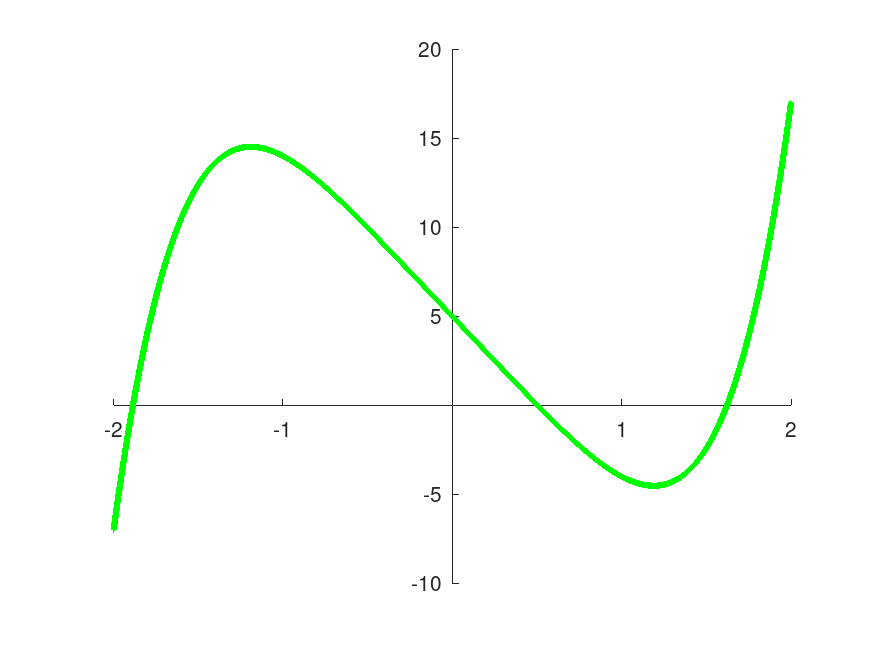
\includegraphics[width=13cm, height=7cm]{quantic2.png}
    \caption{\footnotesize Plotted by the ``GNU-Octave''}
  \end{figure}

 From its graph this polynomial has only three real roots. This polynomial is ``irreducible over \(\mathbb{Q}\) by the Eisenstein's criterion'' \cite{hunger} so by Theorem-11 its Galois group is \(S_5\) which contains \(5!=120\) elements.
 \end{example}

  \begin{tcolorbox}[colback=gray!20, colframe=blue!30, title={\small \bfseries \textcolor{black}{GNU-Octave Code for the above plotting}}, width=15cm]
\begin{boxedverbatim}
  x=-2:0.000001:2;
  y=x.^5-10*x+5;

  plot(x,y,"g","linewidth",3);
  xlabel="x";                     yabel="y";
  title="Graph of the quantic y";
  box off;
  set(gca, 'XAxisLocation', 'origin', 'YAxisLocation', 'origin');
\end{boxedverbatim}
  \end{tcolorbox}

\vspace{5mm}

\begin{example}
  The polynomial is \(f(x)=x^7-2x^5-4x^3+2x^2+4x-2\) which is ``irreducible over \(\mathbb{Q}\) by the Eisenstein's criterion'' \cite{hunger}. Its graph is shown below.

    \begin{figure}[h!]
    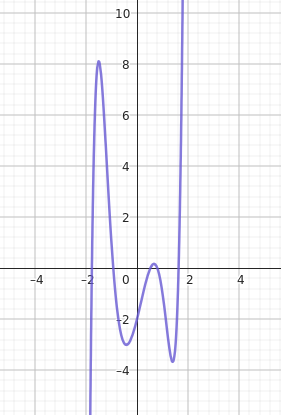
\includegraphics[width=11cm, height=7cm]{seventh2.png}
    \caption{\footnotesize Plotted by the ``Geogebra''}
  \end{figure}
The Graph shows this polynomial has exactly five real roots. So exactly two of its roots are complex. Hence by the Theorem-11 its Galois Group is \(S_7\) which contains \(7!=5040\) elements.
\end{example}

\vspace{5mm}
\section{Galois Group of Reducible polynomials}
For any polynomial \(f \in K[x]\) we factor \(f\) into irreducibles as \(f_1f_2...f_k\) and compute the Galois group \(G_i\)  of \(f_i\) for each \(i=1,2,...,k\). ``Then the Galois group \(G\) of \(f\) is isomorphic to a subgroup of \(\prod G_i\)'' \cite{algorithm}.\\

\begin{example}
  The polynomial is \(f(x) = x^4-7x^2+15\)\\
  Here, \(f(x)=(x^2-3)(x^2-5)\) so it is reducible over \(\mathbb{Q}\). Let \(f_1(x)=(x^2-3)\) and \(f_2(x)=(x^2-5)\). Then \(f_1,f_2\) are both irreducible over \(\mathbb{Q}\).\\

  The splitting field for \(f_1\) is \(\mathbb{Q}(\sqrt{3})\) so its ``Galois group is \({\mathbb{Z}}_2\)'' \cite{hunger}. The splitting field for \(f_2\) is \(\mathbb{Q}(\sqrt{5})\) so its Galois group is also \({\mathbb{Z}}_2\). Now we have the Galois group of \(f\) is a subgroup of \(G={\mathbb{Z}}_2 \times {\mathbb{Z}}_2\). \\

  Since the intersection of \(\mathbb{Q}(\sqrt{3})\) and \(\mathbb{Q}(\sqrt{5})\) is trivial the Galois group of \(f\) is \(G\) itself which is \textit{Klein 4-group}.
\end{example}

\begin{example}
  The polynomial is \(f(x)=x^7-5x^5-10x^3+5x^2+50x-25 \in \mathbb{Q}[x]\). This polynomial factors into irreducibles over \(\mathbb{Q}\) as \((x^2-5)(x^5-10x+5)\).\\
  ``The Galois group of \(x^2-5\) is \({\mathbb{Z}}_2\)'' \cite{algorithm} and of \(x^5-10x+5\) is \(S_5\) from the example-3. Also the roots of \(x^2-5\) are \(\sqrt{5}\) and \(-\sqrt{5}\) which are not the roots of \(x^5-10x+5\) from the its graph figure-4.1, so the intersection of the splitting fields of these two factor polynomials of \(f\) is trivial. Hence the Galois group of \(f\) is \(\mathbb{Z}_2 \times S_5\).
\end{example}

\vspace{7mm}
\section{Galois groups of Multi-variable Polynomials}
The Galois group of a polynomial in single variable can be generalized to the Galois group of a multi-variable polynomial.
\vspace{3mm}

\begin{example}
  The polynomial is \(f(x,y)=x+y \in \mathbb{Q}[x,y]\). The roots of \(f\) spans all over the complex numbers. Hence its Galois group is a subgroup of the symmetric group \(S_{|\mathbb{C}|}\).
\end{example}

\vspace{1mm}
\begin{example}
  The polynomials in \(\mathbb{Q}[x,y]\) are: \begin{align}
                         y &= x^2+1 \\
                         y &=x
                       \end{align}.
                       The roots of these simultaneous polynomials are \(\omega, {\omega}^2\). Then the splitting field of this system is \(\mathbb{Q}(\omega)\). Here the automorphisms of \(\mathbb{Q}(\omega)\) are: \\
       \(\omega \longmapsto \omega\) and \hspace{9mm} \(\omega \longmapsto {\omega}^2\).\\
                       Hence the Galois group of this system is \(\{(1), (12)\} \cong {\mathbb{Z}}_2\).
\end{example}

%%% Local Variables:
%%% mode: latex
%%% TeX-master: "n"
%%% End:
